\myChapter{Evolutionary Algorithms}\label{chap:distributedEAs}
\minitoc\mtcskip
\vfill
\lettrine{E}{volutionary} computation is a wide sub-field of the computational intelligence area, comprising several kinds of algorithms and its variants, techniques and tools \cite{eiben2003chapter1}. This chapter shows a brief revision of the state of the art in this area, showing the most used algorithms, distribution models, and frameworks, to finally explain some of the existent deficiencies to be solved. We also introduce the terminology that will be used in next chapters.  

The term \textsc{Evolutionary Algorithm} is used to describe a computer-based problem solving system that use computational models whose design is inspired by evolution mechanisms. They are based on a \textsc{population} of \textsc{individuals}, where the natural selection, caused by the environmental pressure, leads to an increase of the \textsc{fitness} of the individuals \cite{eiben2010whatis}. This fitness is an evaluation function that describes the quality of the solution of the problem being solved. Individuals within the population are combined and modified by means of \textsc{recombination} and \textsc{mutation} operators, creating new individuals to be added to the population. The general scheme of an EA, extracted from the work of \person{Eiben and Smith} \cite{eiben2010whatis} is described in Figure \ref{fig:basicscheme}.


\begin{SaveVerbatim}{BasicEAtext}
BEGIN
 INITIALISE population with random candidate solutions;
 EVALUATE each candidate;
 REPEAT UNTIL (TERMINATION CONDITION is satisfied) DO
   1 SELECT parents;
   2 RECOMBINE pairs of parents;
   3 MUTATE the resulting offspring;
   4 EVALUATE new candidates;
   3 SELECT individuals for the next generation;
 OD
END
\end{SaveVerbatim}


\begin{SCfigure}[][!hb]
\begin{tabular}{|A|}
\hline
\BUseVerbatim{BasicEAtext}
\\
\hline
\end{tabular}
\caption{General scheme of an evolutionary algorithm in pseudo-code}
\label{fig:basicscheme}
\end{SCfigure}

Also, according to \cite{eiben2010whatis} the features of an EA are:
\begin{itemize}
\item EAs are population based.
\item EAs mostly uses recombination to generate new individual from the existent ones.
\item EAs are stochastic.
\end{itemize}

%During the execution of the EAs, two different phases exist:
%\begin{description}
%\item[Exploration] Generation of new individuals to expand the search space. This is usually performed in the first iterations of the EA.
%\item[Explotation] Concentration in the neighbourhood of the best solutions.
%\end{description}

This chapter introduces a general overview of the most used types of Evolutionary Algorithms to clarify their common elements. Also, the most extended models to parallelize EAs are presented, to understand all their possible architectural possibilities. Finally, some of the most used frameworks to develop EAs are listed and analysed, to summarize their capabilities and lacks. This way, in following chapters, the design of services for EAs will have a solid base to start.

\section{Types of Evolutionary Algorithms}

\lettrine{A}{lthough}  EAs follow the scheme showed in Figure \ref{fig:basicscheme}, they have differences depending on the representation of the solutions, the problems to solve, and other features. This section explains the traditional variants, according to the book of \person{Eiben and Smith} \cite{eiben2003introduction}.

\begin{description}
\item [Genetic Algorithms] These kind of algorithms were proposed by \person{Holland} \citep{holland1975adaptation}, and also studied by \person{Goldberg} \cite{goldberg1988genetic} and \person{Michalewicz} \cite{michalewicz1996genetic}. In this kind of EA, the representation of the solution is a string of numbers (usually binary), called \textsc{chromosome} (and sometimes \textsc{genome}). The individuals are selected proportionally to their fitness, and then \textsc{recombination} and/or \textsc{mutation} are applied to generate new individuals that will be introduced in the population. These algorithms have been used in different areas, such as function optimization \cite{michalewicz1996genetic}, combinatorial optimization \cite{Esparcia2009EVITA}, artificial intelligence in videogames \cite{Fernandez20111optimizing}, or generative art \cite{Garcia2013RGB}, among others. 

\item[Evolution Strategies] The Evolution Strategies (ES) are used to solve problems whose solution is included in the domain of real numbers. Their main difference with GAs is the inclusion of self-adaptation of the mutation rate, being coded in each individual \cite{eiben2005shared}. Also, the parent selection is performed randomly. ES have been applied in fields such as Evolutionary Robotics \cite{Garcia2012testing}.

\item[Evolutionary Programming] In Evolutionary Programming (EP), the representation of the solution depends on the nature of the problem being solved, for example, neuronal networks \cite{Castillo1999gprop} or Radial Basis Functions (RBFs) \cite{Gonzalez2003multiobjective} have been used as individuals.

\item[Genetic Programming] The objective of this technique is to create functions or programs to solve determined problems. Individual representation is usually in form of a tree, formed by operators (or {\em primitives}) and variables ({\em terminals}). These sets are usually fixed and known. The genome size is, therefore, variable, but the maximum size of the individuals is usually fixed, to avoid high evaluation costs. GP has been used to evolve \definicion{LISP}{LISt Processing} programs \cite{Koza1990Tools}, or \definicion{XSLT}{eXtensible Stylesheet Language Transformations} scripts \cite{Garcia2008XSLT}, among others.

\end{description}

Other EAs have been proposed, such as \textsc{Differential Evolution} (DE) \cite{storn1997differential}, \textsc{Estimation of Distribution Algorithms} (EDAs) \cite{larranaga2002estimation} or \textsc{Bayesian Optimization Algorithms} \cite{pelikan2005bayesian}. %SEGURO QUE SON EAS?


%\subsection{Differential Evolution}
%Differential Evolution \cite{} also exploits a population of potential solutions. Three individuals are selected randomly from the population to create \textsc{random noisy vectors}. These vectors are recombined with original random individuals to create the \textsc{trial vectors}. These vectors are compared one by one with the original vector and the better of each comparison is kept for the next generation.

%Table \ref{tab:summaryEAs} shows the main differences between all this types of EAs. Note that we have selected the common features of each algorithm. For example, the replacement in GAs can be different from the generational one, or the representation can also be a real-value vector. 

%\begin{SCtable}[][t]
%\resizebox{11cm}{!}{
%\begin{tabular}{llllll}
%\hline
%				& Genetic algorithm 	 & Evolution Strategy  & Evolutionary Programming & Genetic Programming & Differential evolution  \\
%\hline\hline
%Representation  & Finite alphabet strings & Real-value vectors  & 					& Tree 				& Real-value vectors 	 \\
%Initialization  & \multicolumn{5}{c}{Multi-column} Random, depending of the problem and individual structure	 						 \\
%Selection 	& Fitness proportional 	& Random 				& 						& Fitness proportional & Random to create noisy vectors \\
%Recombination   & Genome crossover		& Genome crossover		& 						& Sub-tree exchange		& Random gene by gene			\\
%Mutation  		& Random 				& Gaussian perturbation	& 						& Random 				& Implicit in the noisy vectors	 \\
%Replacement		& Generational			& ($\mu,\lambda$) or ($\mu + \lambda$) &			& Generational 			& Compared with the original	 \\
%\hline
%\end{tabular}
%}
%\caption{Differences between the types of EAs.}
%\label{tab:summaryEAs}
%\end{SCtable}



Combining elements of previous algorithms with other heuristics are the base of \textsc{Memetic Algorithms} (MAs). These algorithms are based on the concept of \textsc{meme} proposed by \person{Dawkins} \cite{dawkins2006selfish}. A meme is domain specific knowledge coded by a computational representation to the effective solving of a problem. %It is a cultural know-how building-block transmittable and replicable.

This kind of algorithms can be seen as an hybrid combination of the population-based evolution methods previously explained, coupled with some kind of local search. Initially, the hybridization was made just combining two o more methods with some kind of problem knowledge. For example combining a genetic algorithm with Simulated Annealing (SA) \cite{Rodriguez2012Hybrid}. The local search can be performed before, during, or after the evaluation. New trends, such as adaptative MAs \cite{ong2006classification} lead to the usage of several memes for searching and deciding dynamically which meme to apply to each individual. For example, \person{Cowling \etal}�proposed the term \textsc{hyperheuristic} \cite{cowling2001hyperheuristic} as the strategy to choose the meme to be applied depending on the time and the region of the search space (or, in a brief, heuristic to choose memes).  Other examples are the work of \person{Krasnogor \etal} \cite{krasnogor2002multimeme}, where the 
inclusion of the memetic codification inside the individual chromosome (\textsc{Multimemes}) to select which meme to use is applied;  or codify a set of rules, as proposed by \person{Smit} \cite{smith2002co} (\textsc{Co-evolving MAs}). 


\section{Parallel and Distributed Evolutionary Algorithms models}

\lettrine{E}{volutionary} Algorithms are inherently parallelizable. Fitness evaluation can be distributed into several slave machines, or the population can be distributed among different nodes to be evolved at the same time. In 2002, two main types of parallelization models for EAs were classified by \person{Alba and Tomassini} in \cite{alba2002parallelism}: \textsc{Global parallel EAs} and \textsc{Spatially structured EAs}. However, with the aim of new technologies and architectures, such as P2P, new ways to parallelize EAs have been proposed.

\subsection{Traditional parallelization classification}

In this classification, issues such as fault-tolerance, churn, massive scalability or decentralization are not taked into account. The number of computational nodes are fixed during the whole execution and both the network and the nodes are reliable and trustworthy.

\subsubsection{Global parallel evolutionary algorithms}
In this model, also called \textsc{Farming model}, \textsc{Master-Slave} or \textsc{Centralized EA}, the parallelism is applied at evaluation level, where a central node coordinate several slave nodes. The central node executes the EA in a sequential way, but distributes the individuals of the population to the slaves just for being evaluated. Figure \ref{fig:masterslave} depicts this situation.%An example can be seen in \cite{NUCLEAR}, where slave nodes evaluates fitness function for simullation of nuclear devices.

\begin{SCfigure}[20][tb]
\centering
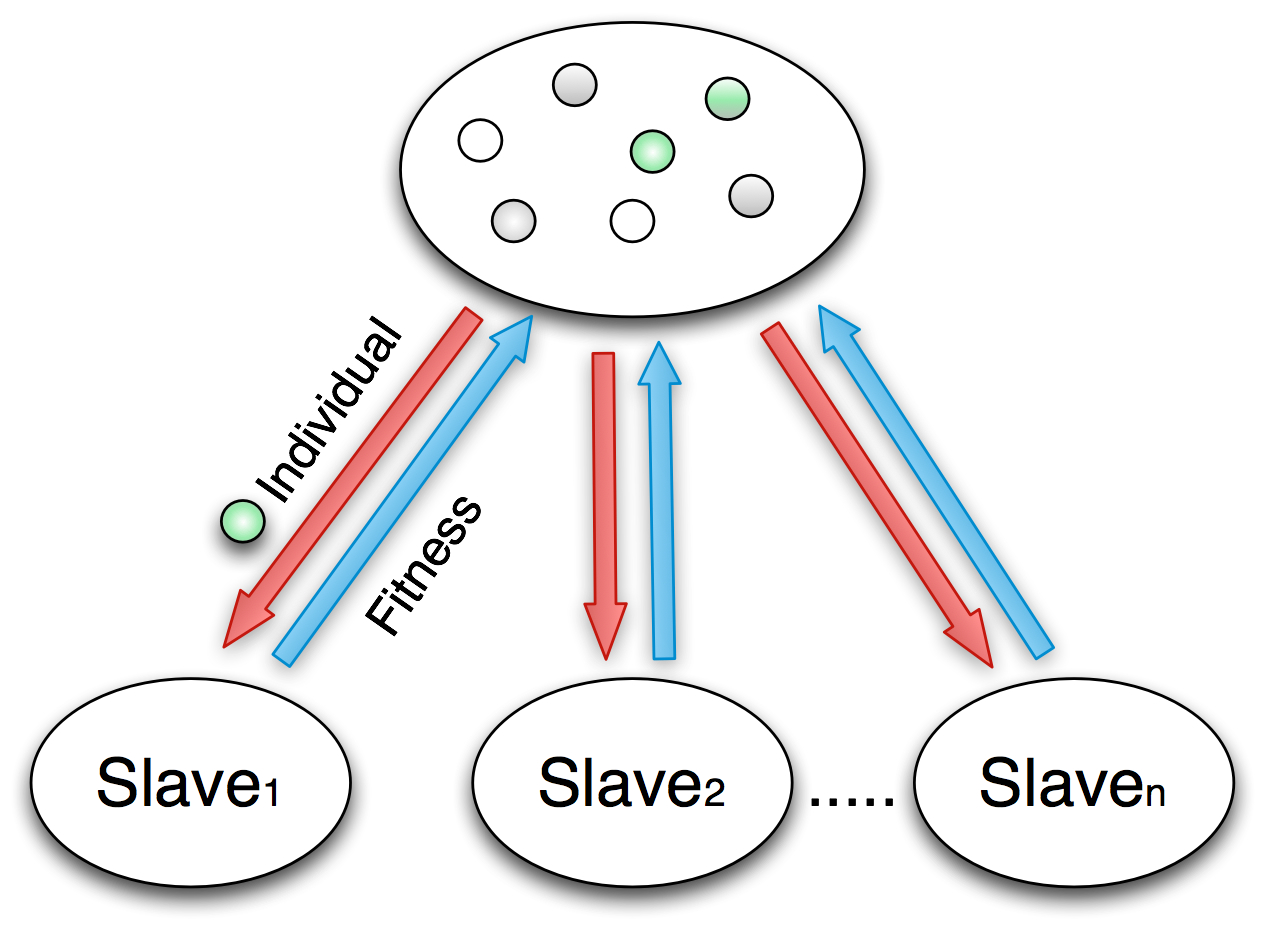
\includegraphics[width=20pc]{gfx/distributed/masterslave.jpg}
\caption{Master-slave model.}
\label{fig:masterslave}
\end{SCfigure}

\subsubsection{Spatially structured algorithms}
The parallelism is performed at population level, that is, dividing the population among the different computing elements. Depending on how the distribution is performed we have:
\begin{description}
\item[Coarse-grained approach] One of the most usual approaches is the \textsc{Island model}, where a number of nodes executes simultaneously the EA, working with different sub-populations at the same time. Each certain number of generations some individuals are interchanged (migrated) between populations. Figure \ref{fig:ring} shows this model with a ring topology.

\begin{SCfigure}[20][tb]
\centering
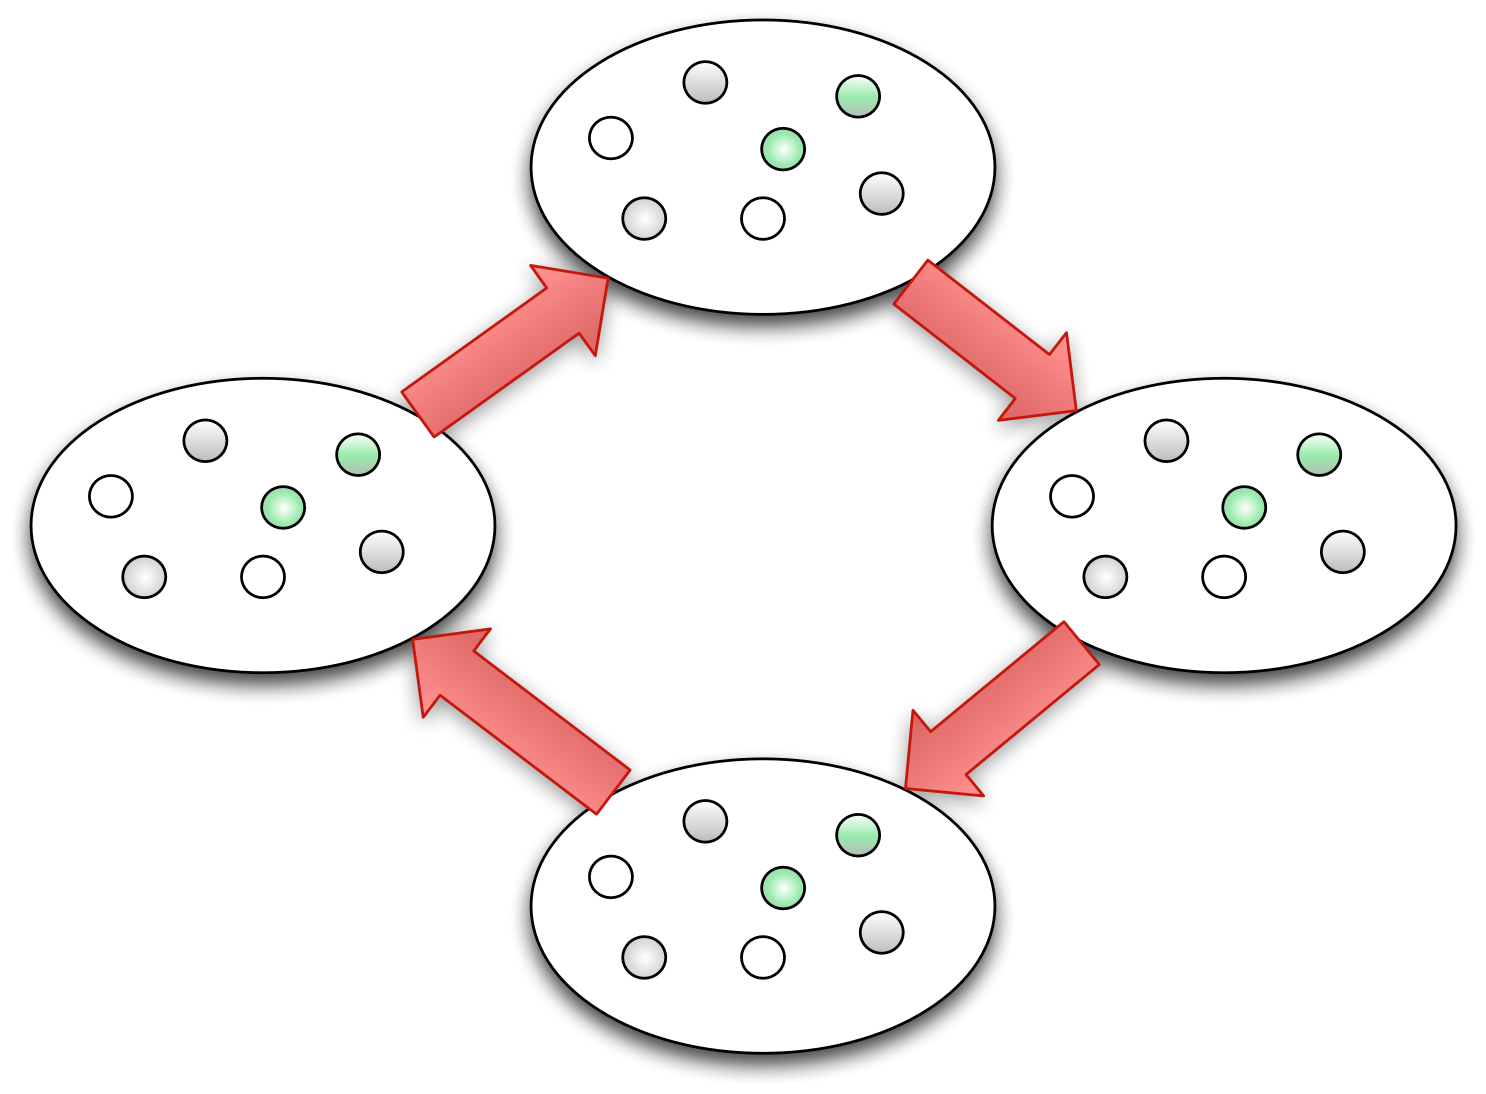
\includegraphics[width=20pc]{gfx/distributed/ring.jpg}
\caption{Island model scheme using a neighbourhood ring topology.}
\label{fig:ring}
\end{SCfigure}

\item[Fine-grained approach] In this approach, also called Cellular EA (CEA), each node has one individual of the population, and selection and reproduction are limited to the individuals of the neighbourhood of the node \cite{CELLULAR}. Usually a bi-dimensional grid is used as topology, such as the one showed in the Figure \ref{fig:cellular}.

\begin{SCfigure}[20][tb]
\centering
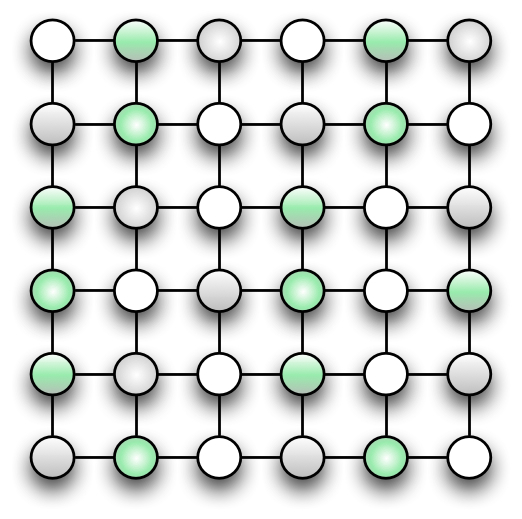
\includegraphics[width=5cm]{gfx/distributed/cellular.jpg}
\caption{Cellular Evolutionary Algorithm.}
\label{fig:cellular}
\end{SCfigure}

\end{description}

\subsection{Non-conventional approaches}
Aside from the previous classification, with the advent of new technologies, such as \textsc{cloud computing}, \definicion{P2P}{Peer-to-peer} networks, or the usage of heterogeneous hardware, new approaches have been proposed. Distributed EAs can be executed in other computing elements different than the classic computers. For example, in mobile devices \cite{Garcia2009Mobile}, ``smart dust'' \cite{Rollings2008smartdust} or inside robots, who on-line learn from the environment \cite{Garcia2012testing}. But with the advancement of the Internet, where hundreds of nodes can co-operate, and whose behaviour is not totally controlled or predicted, is when new distributed approaches have become more evident. 

\subsubsection{P2P evolutionary algorithms}

P2P systems are parallel infrastructures composed by a large number of resources, without any central server \cite{steinmetz2005peer}. The resources in these networks can appear or disappear dynamically. These platforms can be used to execute large instances of problems, taking advantage of the massive scalability that these systems offer. \definicion{EvAg}{Evolvable Agent}�\cite{laredo2010evag} is an EA that uses a decentralized population, where each peer has a single individual, and new individuals are created combining the ones in their current neighbours. The population structure is maintained using the \textsc{newcast} protocol \cite{jelasity2003newscast}: each node has a cache of neighbours that can be interchanged and combined. Figure \ref{fig:evag} shows this algorithm and its population structure. Results show that this algorithm outperforms tuned GAs, using less links that a panmictic (i.e. fully connected) population. 

\begin{SCfigure}[20][tb]
\centering
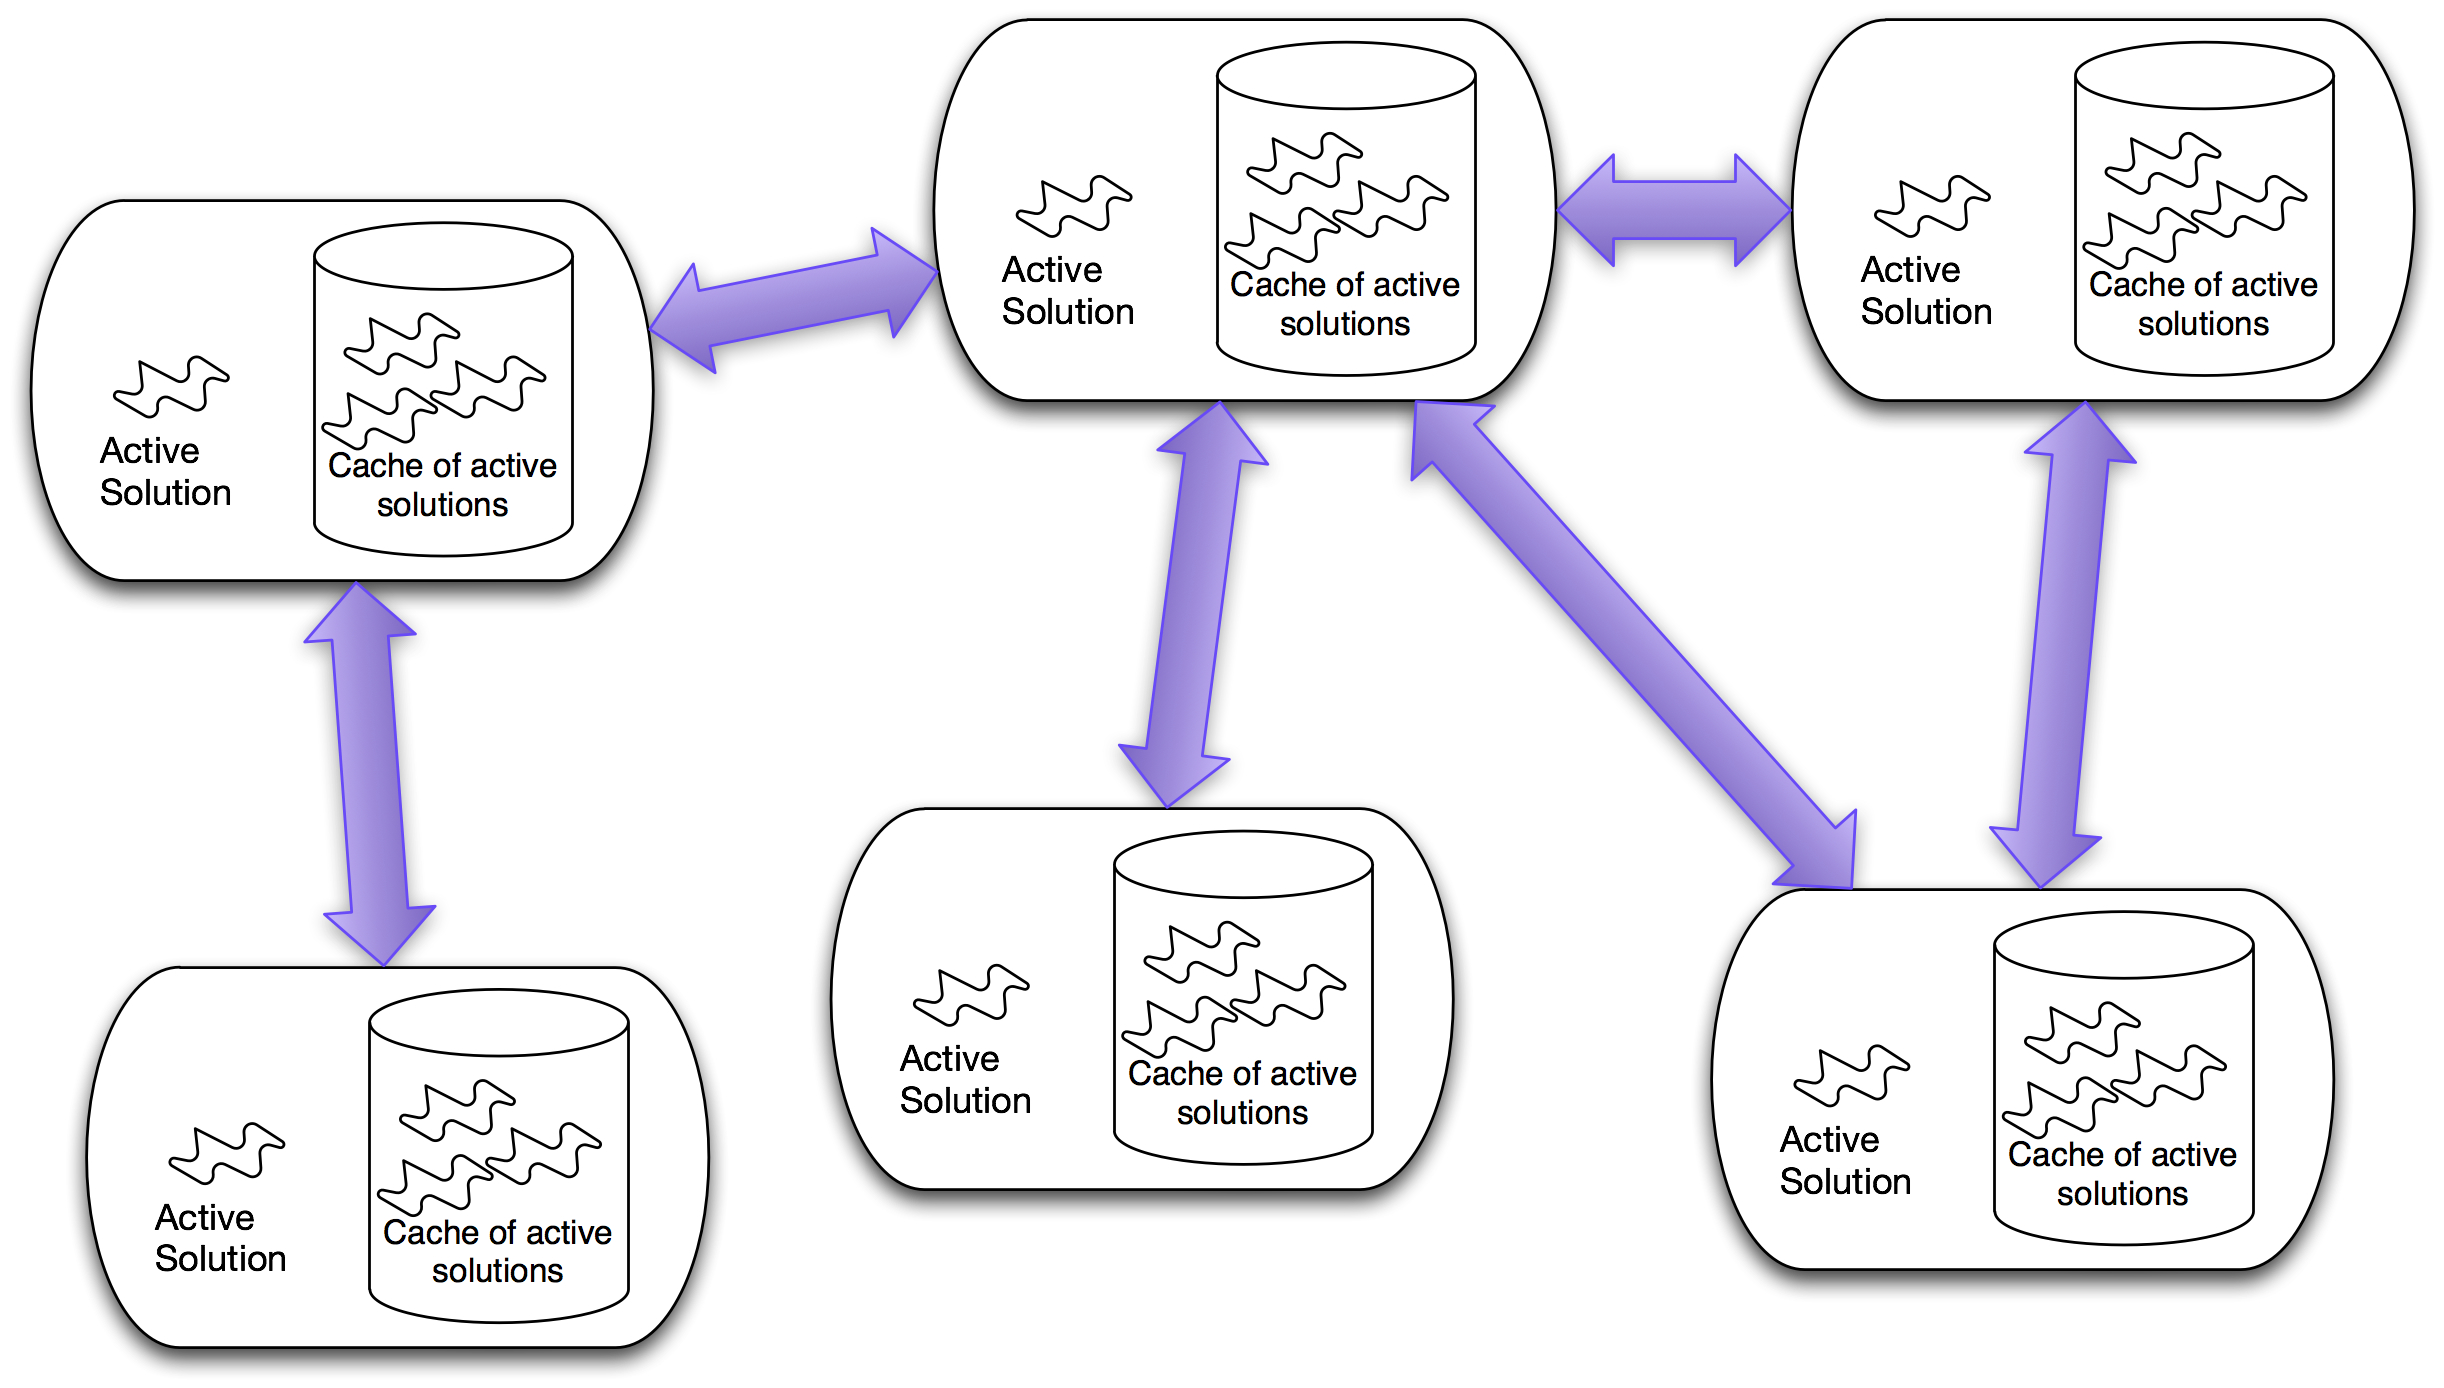
\includegraphics[width=26pc]{gfx/distributed/evag.jpg}
\caption{P2P Evolutionary Algorithm: EvAg.}
\label{fig:evag}
\end{SCfigure}

\subsubsection{Pool-based algorithms}
Other technologies lead to \textsc{Pool-based EAs}, where the computational nodes exchange individuals using a shared pool. This allows massive scalability with a heterogeneous underlying structure. This pool can be used as the global population, and the nodes asynchronously read and evaluate the individuals. Another possibility is that each node behaves as an island and uses the pool to share individuals. This can lead to automatic load-balancing and synchronization, allowing the addition and removal of computers. Different technologies can be used. For example, in the work of \person{Meri \etal},  the pool used is based on the Dropbox\texttrademark\, or SugarSync\texttrademark\, file storage services. Other authors propose the use of non-relational databases, such as the work of \person{Merelo \etal} \cite{merelo2010fluid}, using FluidDB\texttrademark. In \cite{merelo2012pool} the same authors improve the design, proposing an asynchronous, fault-tolerant, and scalable dEA, based on the object store CouchDB\texttrademark. The results show that adding clients could not scale, but increase the fault tolerance. Also, their experimentation shows a good methodology for designing EAs in heterogeneous distributed systems, which have the impossibility of analytic performance prediction.

\subsubsection{Grid and volunteer computing}
Grids are distributed computing systems that allow sharing not geographically centred resources to solve large scale problems. There exist several works that describe EAs being executed in these systems \citep{grid8,grid4,grid10}. \textsc{Volunteer computing} \cite{anderson2005high} proposes the creation of infrastructures to allow people donate CPU cycles for a combined computational effort. Its main difference with grid computing is the presence of un-trusted resources: for example, some nodes could return intentionally wrong results, so it requires possibility of replication. Also, the control of the participating nodes is not maintained by the experiment launcher. EAs have been used in these systems, using different techniques, such as virtualization \cite{Fernandez2013BOINC} or ``parasite'' computing \cite{Merelo2007browser}.


\section{Parameter adaptation in Evolutionary Algorithms}

\lettrine{O}{ne} of the greater challenges of the EC field is to find the appropriate values for EAs parameters \cite{Eiben12Parameters}. Usually, these parameters are established by convection or after several test runs, for example. However, practitioners need to put effort on finding these values in order to attain significant performance in its EAs, even taking into account other variables, such as the computational power of the machines used.

\subsection{Parameter Control and Parameter Tuning}
Two different approaches about the algorithm parameter setting exist in EC: {\em parameter control} and {\em parameter tuning} \cite{ParameterControlEiben99}. The first one refers to setting up a number of parameters of the Evolutionary Algorithm (EA) and changing these parameters in running time. The parameter tuning consist in establishing a good set of parameters {\em before} the run (and do not change these parameters during runtime).

Eiben, in \cite{ParameterControlEiben07} proposes the next taxonomy for the parameter control, according {\em how} are changes made:
\begin{itemize}
\item Deterministic methods: changes to a parameter are triggered by a deterministic rule (for example, increase mutation rate after certain number of generations).
\item Adaptative methods: parameters change depending on some behaviour (for example, increase mutation rate if the average fitness of the population stagnates).
\item Self-adaptative methods: parameters are encoded within the chromosome of the individuals of the population (for example, mutation rate can be a value in the chromosome).
\end{itemize}

Other classifications for control techniques in EAs are presented in that work. For example, regarding to {\em what} is changed:
\begin{itemize}
\item Representation
\item Evaluation function
\item Variation of operators and their rates
\item Selection operators
\item Replacement operator
\item Population
\end{itemize}

Finally, a third classification can be obtained according to what evidence is available:
\begin{itemize}
\item Absolute evidence: The parameter changes if a rule is activated when an specific event occurs. For example: increase mutation rate when diversity drops. In this case, human knowledge is necessary to model these rules.
\item Relative evidence: Parameters are compared with the fitness of their produced offspring and the best values are rewarded. It is not deterministic.
\end{itemize}

\subsection{Adaptation in heterogeneous hardware}

Adapting algorithm parameters to available computational resources leads to improved performance (see the work of \person{Hamadi and Schoenauer} \cite{AutomaticallyConfiguringStyles12}). An easy way to take advantage of the available resources is the load balancing \cite{Garamendi2006Parallel} to distribute workloads across multiple elements. However, assigning equal tasks  to each node on heterogeneous clusters may result in suboptimal performance (as shown by \person{Bohn and Lamont} \cite{LoadBalancingBohn02}). Parameters of an algorithm could also be adapted to increase the performance of the whole system. For example, the population size in EAs is the key to obtain good performance, because it have effect on the quality of the solution and the time spent during the run \cite{ShrinkageLaredo09}. This parameter has been studied as a fixed \cite{SizingHarik99} or adaptive parameter during runtime \cite{AdaptiveLobo07,SelfRegulatedSizeFernandes06}, but without taking into account the computational power of each machine in a heterogeneous cluster. 

The adaptation of an algorithm can be useful to take advantage different hardware environments.
One of the problems in parameter adaptation in heterogeneous clusters is 
the computational load representation. It depends on the algorithm, size of the problem, programming 
language, compiler or hardware characteristics, and the results obtained from artificial 
benchmarks (such as  Linpack \cite{LinpackEndo10}) should not be extolled as identificative 
of the system performance \cite{LinpackDongarra03}. For example, in the work of \person{Garamendi 
\etal} \cite{Garamendi2006Parallel},  a small benchmark was executed in all nodes at the beginning
of the algorithm in order to distribute individuals of an Evolutionary Strategy, following a master-slave model. The computational load by artificial benchmarks may not accurately 
 represent the correct load of the algorithm, so, information 
 about the algorithm itself should be used for calibration.

In other works, there are not direct relation with the algorithm parameters and 
computational resources of the nodes. For example, \person{Dom\'inguez \etal} \cite{Dominguez13HydroCM} 
divided the available devices in ``faster'' and ``slower'' nodes to create a distributed hybrid 
meta-heuristic that combines two different EAs: Genetic Algorithms and Simulated
Annealing. Their system executes the heavy (in computational
terms) algorithms (GAs) in the faster nodes (computational devices), and
simpler meta-heuristics (SA) in the slower ones, obtaining better results
than other configurations.  \person{Gong \etal} in \cite{Gong2005HeterogeneousTopology} also ordered 
the nodes by their computational power to test different topology configurations in a distributed EA.
Besides  ordering the nodes taking into account 
only their previously known computational resources, the results of the previous works were not compared with executions on a homogeneous 
cluster to validate if the adaptation takes advantage of the heterogeneity 
of the cluster.

The heterogeneous computational performance of nodes or network speed can affect the performance of an algorithm. In \cite{Alba2002Heterogeneous},
 \person{Alba \etal} compared a distributed Genetic Algorithm (dGA), one of
 the sub-types of EAs, on homogeneous and heterogeneous clusters. 
 Super-linear performance in terms of iterations was obtained in the heterogeneous ones,
 being more efficient than the same algorithm running on homogeneous
 machines. However, the parameter setting was the same in both
 clusters and they did not adapt the parameters to the machines used.

 Adapting algorithm parameters to computational nodes derives in heterogeneous parameter sets. These sets can improve the results in homogeneous hardware, for example, setting a random set of parameters in each homogeneous node can also increase the
performance of a distributed Genetic Algorithm, as explained by \person{Gong
and Fukunaga} in \cite{Gong2011HeterogeneousParameters}. That model
outperformed a tuned canonical dGA with the same parameter values in
all islands. Also, adapting the migration rate produced better
results than homogeneous periods, as explained by \person{Salto and Alba} in
\cite{Salto2012HeterogeneousMigration}. This indicates that heterogeneous parameters
 may lead to an increase of performance, so it is necessary to validate if the 
 performance is due to the parameter set or to the heterogeneous devices combination.


\section{Frameworks for Evolutionary Algorithms}
\lettrine{T}{here} exist a large number of frameworks for Evolutionary Algorithms freely available for download. Practically every programming language has its own implementation of the basic elements that form an EA. This implies a large effort made in each one, giving that these elements are not compatible among them. It is also difficult to migrate the code from a framework to another, mainly due to design choices, such as the existence of hidden global variables or language specific features (such as functional programming \cite{Cruz2013Erlang}). 

 

\subsection{Object Oriented Frameworks}
There exist many
Object Oriented frameworks, such as Al\-go\-rithm::Evo\-lu\-tionary \cite{PERL}, \definicion{METCO}{Metaheuristic-based Extensible Tool for Collaborative Optimization} \cite{Leon2009metco},
\definicion{JCLEC}{Java Class Library for Evolutionary Computation} \cite{JCLEC} or jMetal \cite{JMETAL}. 
 Users implement specific interfaces of these frameworks ({\em
   individual} or {\em crossover}, for example) and they group them in the source
 code. For example, creating an operator object that groups several
 operators. However, these frameworks are not compatible among them.
 For example, the operators created in JCLEC can not be used in jMetal
 (despite both are programmed in Java). %Also, they can not control the
 %services (operators) outside the source code.

\subsection{Parallel frameworks} 
Parallelism and distribution are possible in other frameworks, such as
MALLBA \citep{MALLBA}, \definicion{DREAM}{Distributed Resource Evolutionary Algorithm Machine} \citep{DREAM} or \definicion{ECJ}{Evolutionary Computation in Java} \citep{ECJ}, but
using external libraries (such as \definicion{MPI}{Message Passing Interface} or \definicion{DRM}{Distributed Resource Machine}), so the code that uses these
libraries is mixed with the algorithm's code.


 Even being distributed, these frameworks can not communicate with each other. HeuristicLab \citep{HEURISTICLAB} is one of the few plug-in and service oriented frameworks. It uses web services for communication, but just to distribute the load, after consulting a central database of available jobs. Finally, %the only service oriented optimization framework is
 gridUFO is a service oriented framework \citep{gridUFO}, but it only allows the modification of the objective function and the addition of whole algorithms, without combining existing services.  Table \ref{tab:frameworks} shows a summary of the previous frameworks.


\begin{SCtable}[][t]
\resizebox{11cm}{!}{
\begin{tabular}{llllll}
\hline
\rowcolor{colorCorporativoSuave}Name		&  Design 	 & Language 	& Distribution 	& License  		& Last version	\\
\hline\hline
\rowcolor{colorCorporativoMasSuave}ECJ		& OO		& Java		& Sockets   	& Academic Free Lic. 	& 2013		\\
\rowcolor{colorCorporativoSuave}MALLBA		& OO		& C++		& MPI		& Freeware		& 2010	\\
\rowcolor{colorCorporativoMasSuave}jMetal		& OO		& Java		& N/A		& GNU/LGPL 		&2013		\\
\rowcolor{colorCorporativoSuave}DREAM		& OO		& Java		& DRM		& GNU/GPL   		& 2003		\\
\rowcolor{colorCorporativoMasSuave}ParadiseEO	& OO		& C++		& MPI		& CeCILL	   	& 2012		\\
\rowcolor{colorCorporativoSuave}HeuristicLab	& OO/PO 	& .NET		& Web-Services	& GNU/GPL		& 2013			\\
\rowcolor{colorCorporativoMasSuave}METCO		& OO		& C++		& MPI		& N/A	   		& 2009	\\
\rowcolor{colorCorporativoSuave}JCLEC		& OO		& Java		& N/A		& GNU/GL   		&	2013 \\
\rowcolor{colorCorporativoMasSuave}Algorithm::Evol.& OO		& Perl		& N/A		& GNU/GPL  		& 2013	\\
\rowcolor{colorCorporativoSuave}gridUFO		&SO		& Java		& Web Services	& N/A  			& 	2010 \\
\hline
%OSGiLiath	&OO/SO/PO 	& 2010			& Java		& Distributed OSGi	& GNU/GPL  	& Lifecycle management	\\
\end{tabular}
}
\caption{Comparison of EA frameworks. OO=Object-Oriented, SO=Service Oriented, PO=Plug-in Oriented}
\label{tab:frameworks}
\end{SCtable}

In brief, although these frameworks follow the six criteria for genericity 
proposed by \person{Gagn{\'e} and Parizeau} in \cite{GENERICITY05}, they present some shortcomings when it is needed to develop
or add new features: the user is forced to modify the source code
or stop the execution to add new functionalities (like load balancing,
dynamic control of operators, or an user interface).


\subsection{Volunteer computing frameworks}

%As previously said, there exist authors describing EAs being executed in grids \citep{grid8,grid4,grid10} and a frea

\definicion{BOINC}{Berkeley Open Infrastructure for Network Computing} is one of the most used frameworks in volunteer computing. This middleware follows a master-slave architecture, where the server is in charge of hosting the project experiments and the creation and distribution of jobs \cite{Fernandez2013BOINC}. Clients ask the server for works, download information, compute data and upload the results. EAs have been used in BOINC, such as the work of \person{Fern\'andez \etal} \cite{Fernandez2013BOINC}. Other authors imitate this architecture using a browser-based scheme \cite{Merelo2007browser} to distribute fitness evaluations among clients without installing any other software.

Previous systems have the possibility of task distribution among the nodes, following a master-slave model, but without interaction between clients.

\subsection{Design of EAs}
The work of \person{Gagn\'e and Parizeau} \cite{GENERICITY05} established six criteria to qualify the genericity of a framework for EAs. 

\begin{itemize}
\item Generic representation: independence of the structure of the individuals. 

\item Generic fitness: Individual fitness should be as independent as possible from the selection operators and individual representation. That means that the fitness evaluation should be outside of the implementation of the individuals (for example, not implementing the fitness in the class that implements the individual). 

\item Generic operations: operations should be used in conjunction with others and have minimal side effects. For example, a multi-parent reproduction (crossover with more than two parents, as presented by \person{Eiben et al.} \cite{EibenMultiparent97}) requires separation of the concept crossover with only two elements, so the abstract concept of crossover  should accept a list of individuals. Also, new operations can be created without affect the existent ones, allowing the interaction of a non-limited number of operators. Finally, the granularity of the design of the operators must be equilibrated, not being neither too coarse (may limit the flexibility to create new operators) nor too fine (could be difficult to integrate all the operators).

\item Generic evolutionary model: As explained before, there exist different ways to model an EA leading to different algorithms (for example, a steady-state GA versus a generational GA, or a GA versus ES). Operators should be independent of the evolutionary model, being possible the change from a model to another. 

\item Parameter management: parameters, such as the population size, may be modified during runtime. Also, a good framework must accept the addition of new parameters.

\item Configurable output: the output should be configurable. This is due to different statistics that could be used depending on the EA: for example, the tree depth in GP. Also, different outputs (console, files) should be managed.



\end{itemize}


\section {Conclusions}
\lettrine{E}{volutionary} Algorithms, and their subtypes (GAs, ES or GP, among others) follow a number of common steps: initialization, evaluation, selection, recombination, mutation, replacement and stop criterion. There exist many variations of these steps, and the different combinations can specify one algorithm or another. Memetic Algorithms also include extra elements that can be applied, and different heuristics can be combined during the algorithm's run.

Distributed EAs can improve the algorithmic and computational performance. Classic parallelization approaches, such as the master-slave or island-based models, have been updated with the usage of new trends such as P2P or pool-based EAs. These new approaches manage with computational nodes entering and exiting during the experiment runtime and heterogeneous architectures.

Other research lines, such as the parameter adaptation can imply the existence of some kind of dynamism involving the parts that compose an algorithm: for example, different recombinators or mutators working at the same time. Moreover, there exist several lines of parameter adaptation in dynamic and heterogeneous environments, where different computational elements are working at the same time.

Finally, there exist a large number of different (and incompatible) frameworks for EAs, each one using different languages, technologies and communication protocols. As \person{Parejo \etal}  suggest  in \cite{SURVEYMOFS}, a standardization of the presented (and other) frameworks should be carried out. Moreover, it is difficult to access, in a public way, to available public systems to execute existent EAs to validate experiments and save time, encouraging open science.

Next chapter will explain a possible technological solution to address previous issues.
